\section{Modelling}

\begin{frame}{MLS Model}

    One of the main challenges of this project is to correctly model the interactions between the ball and the electromagnets.

    To this aim, we have started from the energy conservation principle and model the system via Lagrange's equations:

    \begin{equation}
    \begin{cases}
        \dot{z} = v \\
        \dot{v} = m^{-1} \left( \frac{1}{2} \frac{\partial L_1}{\partial z} I_1^2 + \frac{1}{2} \frac{\partial L_2}{\partial z} I_2^2 + m g \right) \\
        \dot{I_1} = L_1^{-1} \left( -R_1 I_1 + V_1 + R_1 I_{1_{\text{min}}} \right) \\
        \dot{I_2} = L_2^{-1} \left( -R_2 I_2 + V_2 + R_2 I_{2_{\text{min}}} \right)
    \end{cases}
    \label{eq:reduced_equations_of_motion_final}
\end{equation}

\end{frame}


\begin{frame}{Electrical components modelling}

    What we are trying to achieve now.

    \begin{figure}
        \centering
        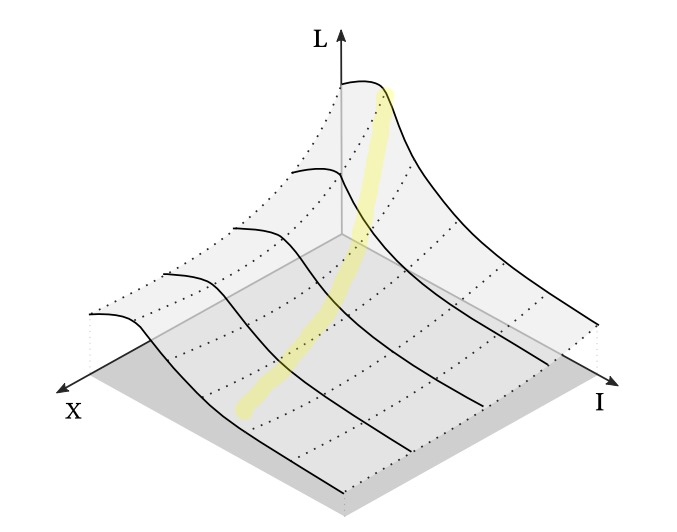
\includegraphics[width=0.8\textwidth]{img/inductance_curve.jpg}
        \caption{Inductance dependence over ball's position and current}
    \end{figure}

\end{frame}